%Chapter 3
Predicting disorder from XANES spectra requires a sophisticated model or algorithm capable of extracting non-linear features from the data. Increasing the disorder in the structure does not simply shift or scale the spectrum by a scalar; instead, disorder alters the spectrum in a complex and unknown way, for which we rely on machine learning  (ML) to discern. The general goal of ML is to recognize patterns in data, iteratively learning to solve complex, non-linear problems and make powerful predictions on new, unseen data \cite{ML-and-the-physical-sci}. Due to the integral role ML plays in this thesis, the following chapter serves to establish how neural networks fundamentally operate, and define all the terms necessary for understanding the neural network implementation discussed in chapter \ref{ch:results}.

We begin by clarifying and distinguishing the following commonly misused terms: machine learning (ML), deep learning, and artificial intelligence (AI). ML is the most general term out of the three, referring to the computational technique of fitting a model on a dataset via an iterative training process. The models created in ML can either be regressors or classifiers: the former predicts a continuous range of values, whereas the latter is a discrete predictor. Artificial Neural networks (ANNs), or neural networks (NN) for short, are one example of a machine learning model that tends to be complex and computationally intensive to train. As a result, NNs are often highly non-linear models capable of solving complex tasks such as object detection \cite{szegedy2013deep} or speech recognition \cite{ms-speech-recognition-paper} \cite{speech-recognition}. Neural networks were inspired by biological nervous systems. Fittingly, graphical representations of ANNs include terms such as ``nodes'' and ``connections.'' The field of ML involving ANNs with many layers is referred to as deep learning \cite{schmidhuber2015deep}. AI is a subfield of deep learning where a neural network is trained to generate human-like responses. Common examples of AI are generative chatbots \cite{chatbots} and a virtual assistants \cite{virtual-assistants} \cite{virtual-assistants2}. 

Using the above terminology, we can reframe the goal of this thesis: to predict disorder from XANES, we utilize deep learning to train a regression-based artificial neural network. The following sections walk through the mathematical process of training a simple neural network. In practice, sophisticated APIs such as Google's TensorFlow \cite{tensorflow2015-whitepaper} or Facebook's PyTorch \cite{pytorch-paper} handle the mathematical backend and optimization; however, one must first build a fundamental understanding of the methods these frameworks are executing before attempting to implement them.

\section{Feedforward and Backpropagation in ANNs}

% Understanding how a neural network makes a prediction requires a solid grasp of linear algebra. 
The process where an ANN passes information from the input to the subsequent layers to make a prediction is called the ``feedforward process.'' The name comes from the operation where each layer of the ANN passes information to the next layer until the output layer is reached and a final prediction is made. The process of updating the parameters of a neural network is called backpropagation. Whereas feedforward is essentially a chain of linear algebra operations, backpropagation relies principally on vector calculus. Neither action is particularly mathematically complicated; however, there are many parts, and it is easy to get lost in the sea of similar-looking partial derivatives. In this next section (\ref{sec:feedfoward}), we explicitly walk through the mathematics of the feedforward process for a fully connected (affine) neural network.

\subsection{Feedforward} \label{sec:feedfoward}
Consider the neural network in Figure \ref{fig:simpleNN}: it contains an input layer with three nodes, a single hidden layer with five nodes, and an output layer with two nodes. The input layer (zeroth layer) has a cardinality of $ \mu=3 $ and is represented in Einstein notation\footnote{Recall that in Einstein notation repeated indices are implicitly summed over. For example, ${u^i = A^i_j x_j = \sum_{j=1}^5 A_{ij} x_j}$ } as the covector (row vector) $ x_\mu $. Each edge in the graph represents a weight that will be multiplied by the connecting node on its left in the feedforward process. First, each node in the input layer is multiplied by the weight of the connecting edge and added together. Applying this operation for all input nodes and weights can thus be represented as the inner (dot) product of the input layer row vector and a weights matrix. The hidden layer (first layer) has a cardinality of $ \nu=5 $. Thus, the resulting inner product is $ x_\mu W_\nu^{\mu(1)} $, where $ W_\nu^{\mu(1)} $ represents the matrix of weights connecting the zeroth and first layer. While this result has the correct dimensionality for the hidden layer, there are still two operations required to produce the actual values for the nodes $ h_\nu^{(1)} $. First, a small trainable parameter, $ b_\nu $  is added to every element in the resulting vector from the previous calculation. The values in this row vector are called biases and introduced to prevent overfitting---i.e. the phenomenon where a model predicts the training data well but does not generalize and reliably predict unseen data. Biases are a regularization parameter. Regularization techniques are discussed below and an example is provided in Figure \ref{fig:overfitting}. The final operation applied to produce the first hidden layer's values is known as an activation function. These functions are applied element-wise to the layer, and without them, neural networks would be unable to learn non-linear features. There are several types of activation functions, the three most common being sigmoid, $\tanh$, and ReLU.


\subsubsection{Sigmoid and Tanh}
The sigmoid and tanh activation functions are defined as the following:
\begin{equation}
    \label{sigmoid}
    \sigma (x) = \frac{1}{1 + e^{-x}}
\end{equation}

\begin{equation}
    \label{eqn:tanh}
    \tanh(x) = \frac{e^x - e^{-x}}{e^x + e^{-x}} 
\end{equation}

\noindent Note, sometimes the term ``sigmoid'' is used to refer to the shape an s-shaped curve, so both equations (\ref{sigmoid}) and (\ref{eqn:tanh}) are considered sigmoids. In machine learning, however, the sigmoid activation function always refers to equation (\ref{sigmoid}). Note that the sigmoid activation function maps the input between zero and one. Hence, the sigmoid often used in the final layer of ANNs to output a probability. The sigmoid function approaches 1 and -1 around $ {x=4} $ and $ {x=-4} $ respectively, meaning that the sigmoid activation function is only useful within that limited range. One issue with both the sigmoid and tanh activation functions is the potential for creating a vanishing gradient. The gradient of either of these functions approaches zero for values above four. This asymptotic approach hurts the ability of the NN to meaningfully update its trainable parameters  \cite{nn-regularization}. The importance of calculating the gradients of these activation functions will be discussed in section \ref{sec:backprop} within the context of backpropagation. 

\begin{figure}[h!]
    \centering
    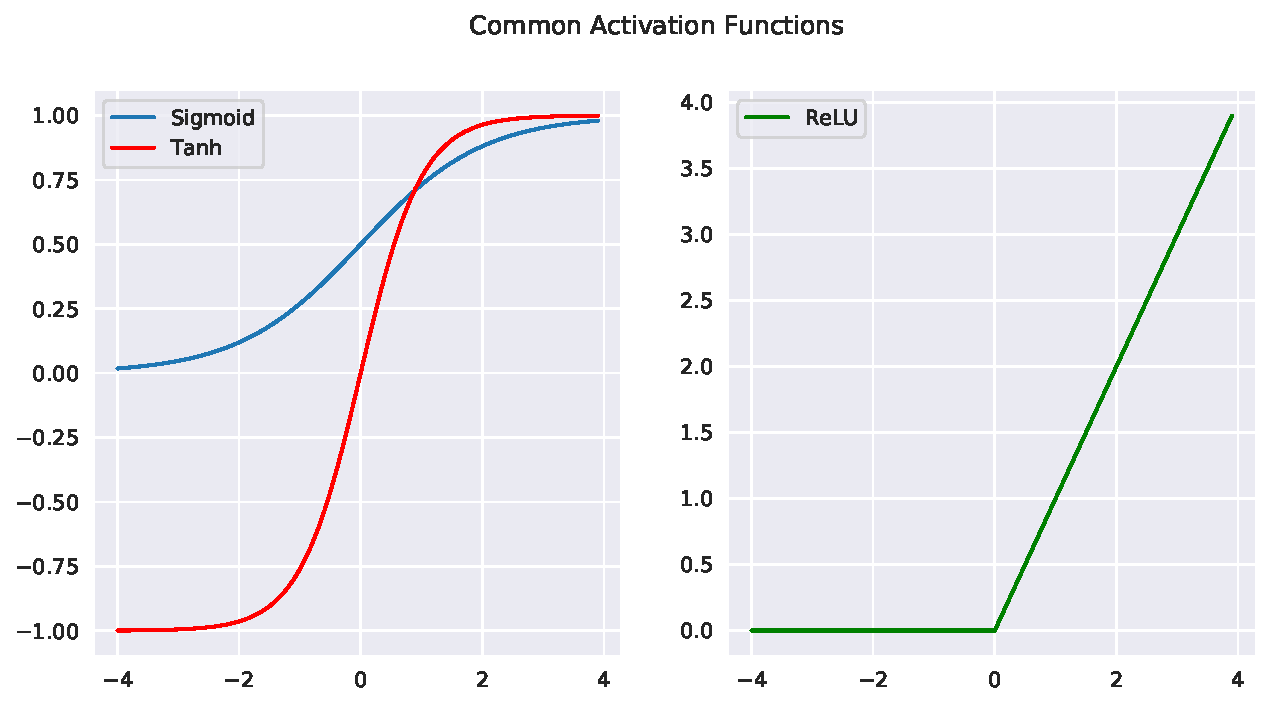
\includegraphics[width=\linewidth]{Chapters/Figures/sigmoids2.pdf}
    \caption[Activation-Functions]{Plotted above are three common activation functions: sigmoid, $\tanh$, and ReLU. Simgoid and tanh are particularly useful for scaling the output of a neural network layer to be within a given range. ReLU and its variations are useful for deep ANNs, where vanishing gradients are problematic.}
    \label{fig:ActivationFunctions}
\end{figure}

\subsubsection{ReLU}
The \textbf{Re}ctified \textbf{L}inear \textbf{U}nit activation function (ReLU) has become an important staple of machine learning. Conventially, it is written as $ f(x) $ and defined as:
\begin{equation}
f(x)=
\begin{cases}
    0 & \text{if } x <= 0 \\
    x & \text{if } x > 0
\end{cases}
\end{equation}

\noindent ReLU is important because it provides a much greater range in values as outputs. Whereas the sigmoid and $\tanh$ activation functions saturate around 4, ReLU never saturates for linear values. Additionally, ReLU is simple to calculate and tends to help neural networks converge quickly. Further, because ReLU returns 0 for any negative value fed forward into the node, many ReLU activation functions in a given layer help lead to sparser layers, reducing the overall complexity of the model and helping prevent overfitting. Arguably its greatest benefit is the reduced likelihood of creating a vanishing gradient \cite{orig-relu}. 


\begin{figure}[h]
    \centering
    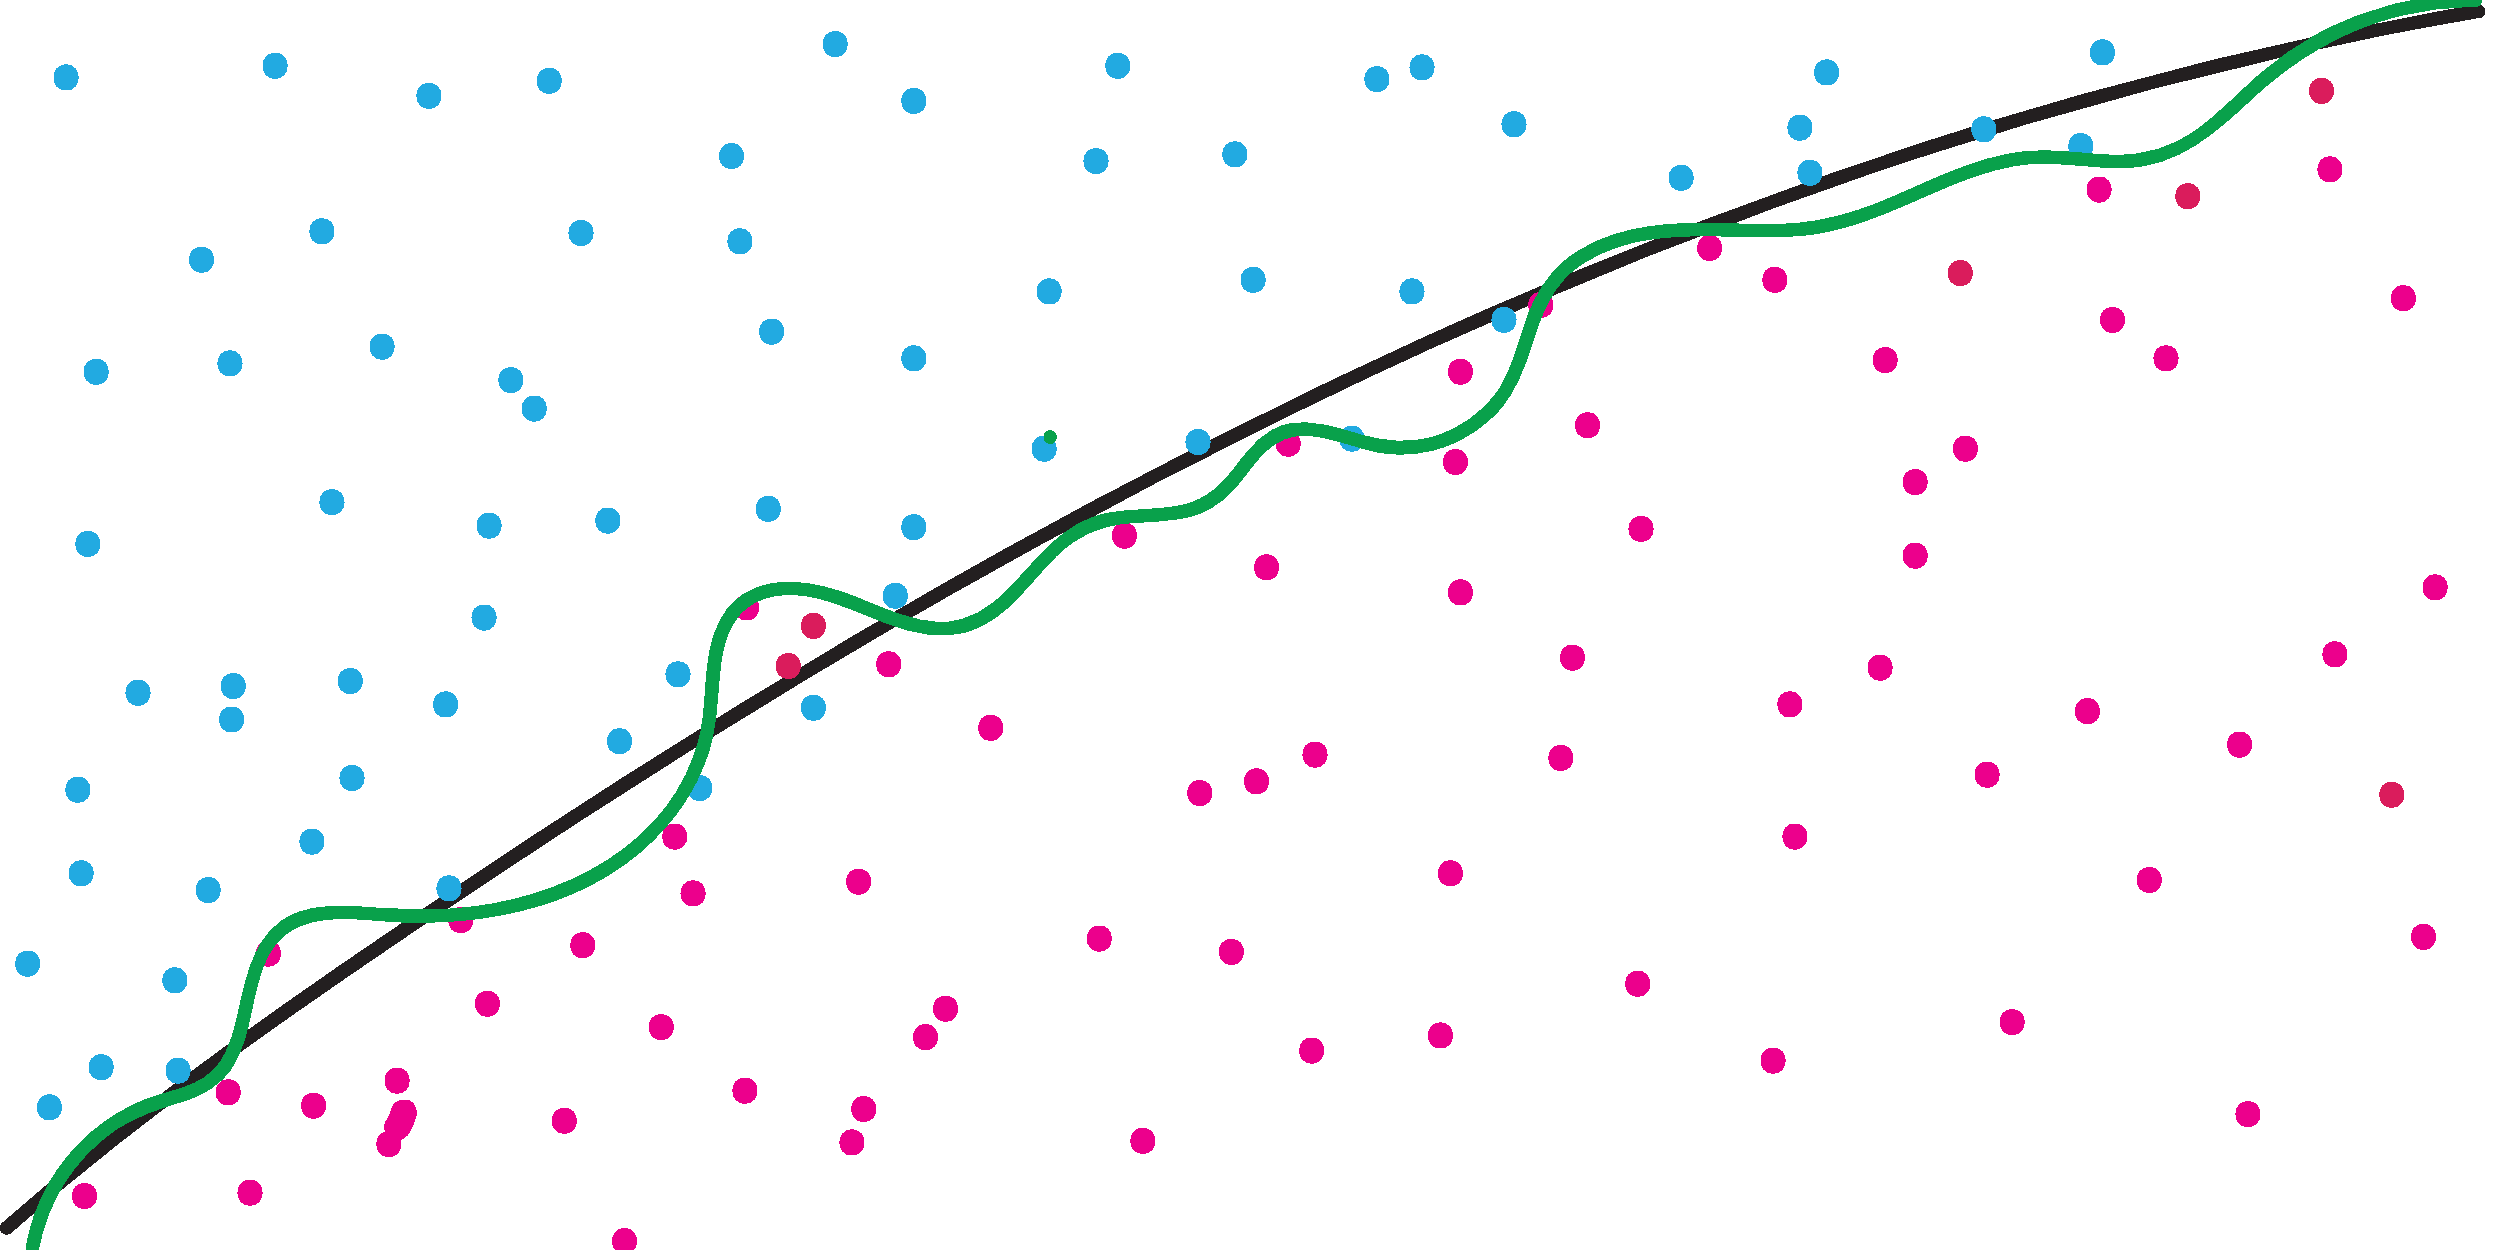
\includegraphics[width=\linewidth]{Chapters/Figures/overfittingOrig2.pdf}
    \caption[Overfitting]{The green curve represents a model overfitting a binary classification problem. Although it makes near-perfect predictions for the training data in this figure, the model will not generalize as well as the simpler black curve when it tries to predict new, unseen data. Introducing biases and dropout layers in neural networks are strategies to prevent overfitting to reduce the model variance and fit the data like the black curve.}
    \label{fig:overfitting}
\end{figure}


With the input nodes dotted with the weight matrix, the baises added, and then the activation function applied to each node, we arrive at the final final vector for the first hidden layer: $ h_\nu^{(1)} $ . Mathematically, $ h_\nu^{(1)} = \sigma\left( x_\mu W_\nu ^\mu + b_\nu \right) $. To calculate the next layer, the process is now repeated---only $ h_\nu^{(1)} $ is used instead of the input layer, and the output
$ \hat{y} = \sigma \left( h_\nu^{(1)} W_\kappa ^\nu + b_\kappa \right)$ is the final output of the neural network. The equations for each step as well as the dimensionality of each layer can be found in Figure \ref{fig:simpleNN}.

\begin{figure}[h!]
    \centering
    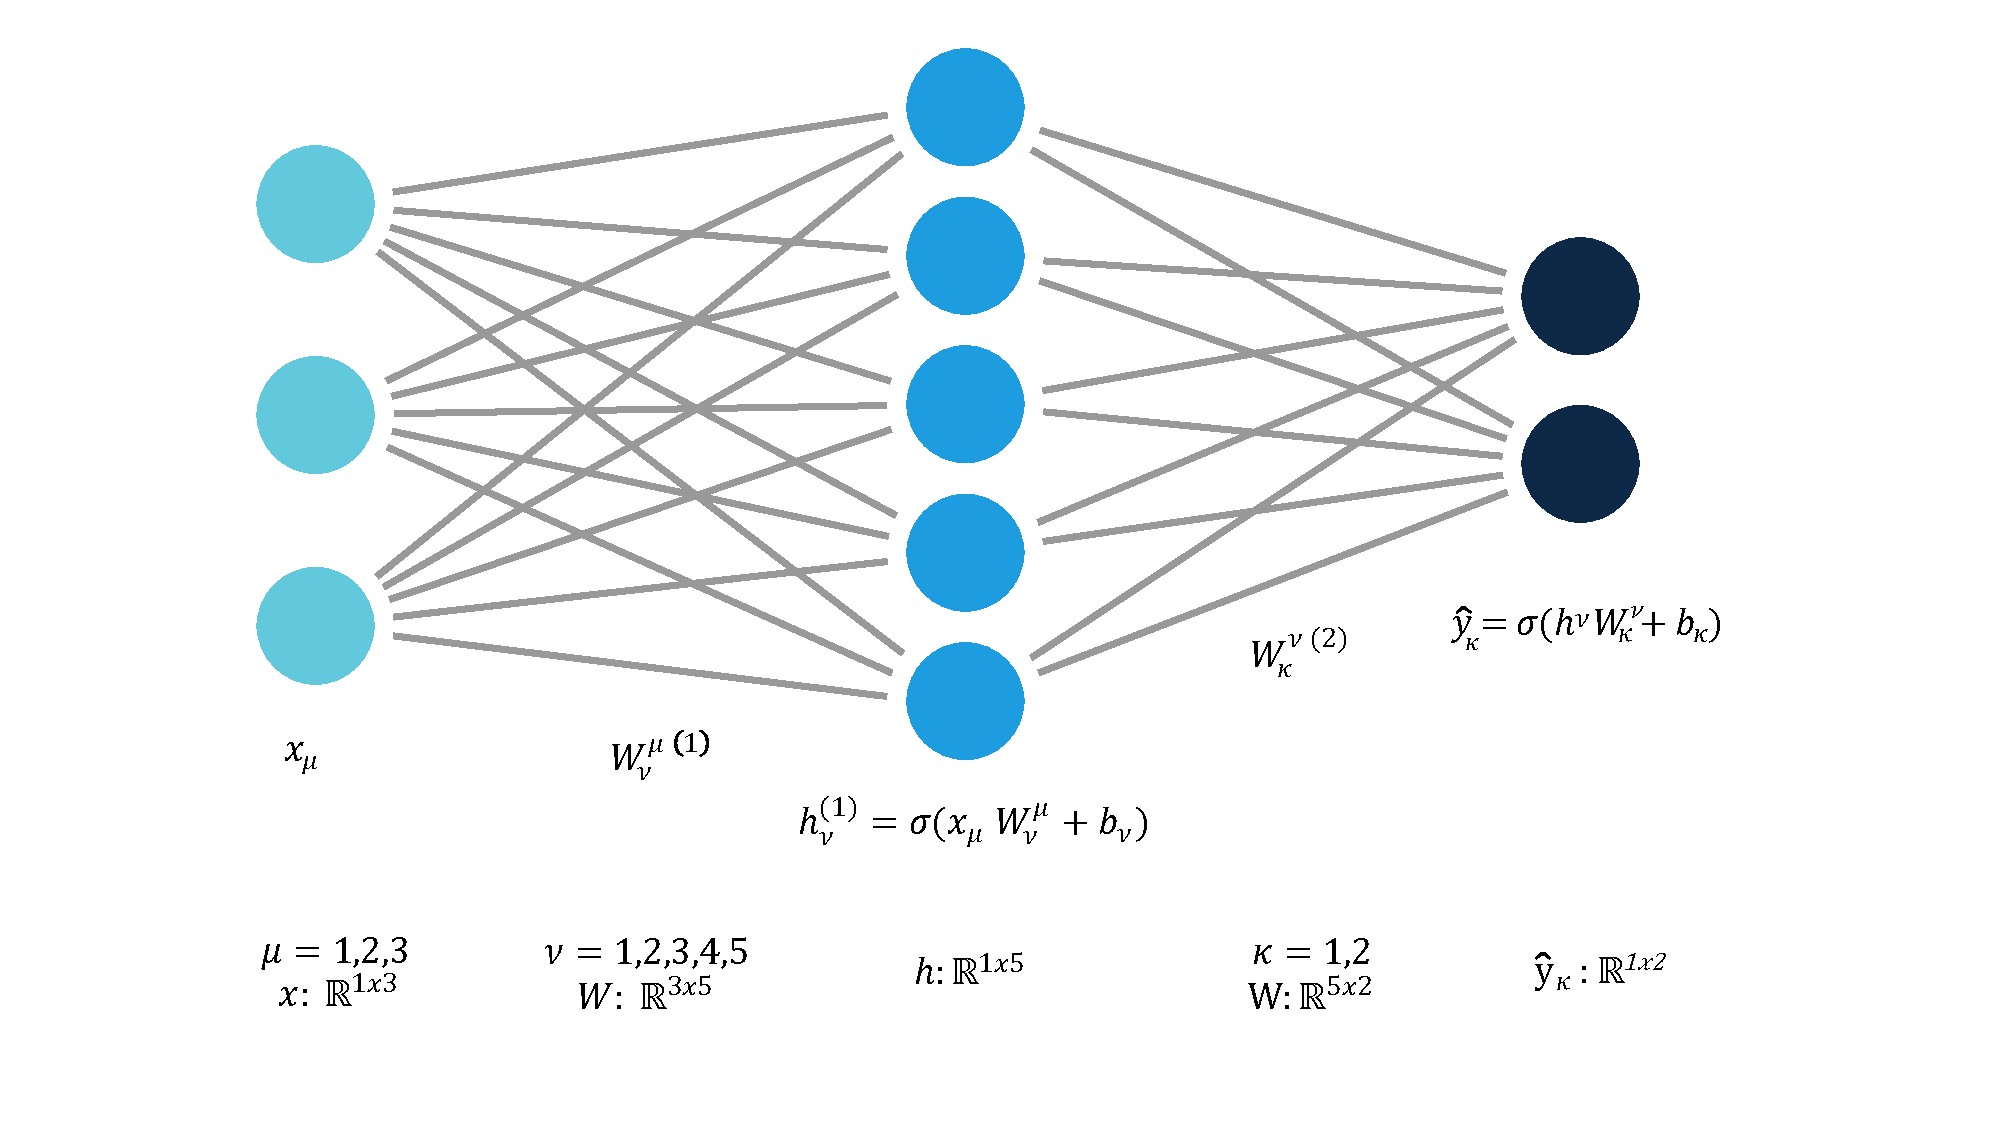
\includegraphics[width=\linewidth]{Chapters/Figures/einstein_NN_2.pdf}
    \caption[Neural Network Example]{This diagram of a fully connected (affine) neural network has a single hidden layer and two output nodes. The tensors for each hidden layer are written in Einstein notation. The implicitly summed over greek letters and dimensionality are written below the tensors for clarification.}
    \label{fig:simpleNN}
\end{figure}

\subsection{Loss Metrics and Regularization}
In order to update the network parameters, it is necessary to evaluate the quality of every prediction the neural network makes. The measure of error for prediction is referred to as the \textit{loss}, whereas the summed total of all the losses is called the \textit{cost}. For regression problems, the two most common cost functions are the mean squared error and the mean absolute error \cite{regularization-2017survey}. Without regularization, they are defined as

\begin{align}
    \label{eqn:lossFunctions-no-reg}
    \text{MAE} &= \frac{1}{n} \sum_i \abs*{\hat{y_i} - y_i} \\
    \text{MSE} &= \frac{1}{n} \sum_i \left( \hat{y_i} - y_i \right)^2
\end{align}

\noindent where $ n $ is the number of training samples. Either cost metric can be regulated. The two most common regularizations are L1 (LASSO) and L2 (Ridge). Applied to the MSE, equation (\ref{eqn:lossFunctions-no-reg}) with regularization becomes: 

\begin{align}
    \label{eqn:lossFunctions}
    \text{L1 MSE: } J &= \frac{1}{n} \sum_i (\hat{y_i} - y_i)^2 + \lambda \sum_j \abs*{W_j}\\
    \text{L2 MSE: } J &= \frac{1}{n} \sum_i \left( \hat{y_i} - y_i \right)^2 + \lambda \sum_j (W_j)^2
\end{align}

\noindent where $ W_j $ is the $ j^{th} $ weight for training sample \textit{i}. 

One simple equation\footnote{This is a simple version of stochastic gradient descent, which will be discussed in depth in section \ref{sec:optimizers} } for updating the weights for loss L is as follows:
\begin{equation}
    W := (1-\alpha \lambda)W - \frac{\partial L}{\partial W}  
\end{equation}

\noindent where $\alpha$ is the learning rate, and $\lambda$ is the regularization hyper-parameter. L2 regularization is often referred to as weight decay. Every iteration, the weights are pushed closer to zero due to the multiplication of the weights by a value $<1$. L1 is known as LASSO (least absolute shrinkage and selection operator), because it shrinks the less important features' coefficients to zero. This is because for small values $\abs*{W_i}$ is a much stiffer penalty than $W_i^2$. Thus, L1 is a good choice when there are dozens of features \cite{nn-regularization}. 

% \noindent Explicitly, for one component of the hidden layer:

% \begin{align}
%     h_j &= \sigma(w_{1j}x_1 + w_{2j}x_2 + w_{3j}x_3 + w_{4j}x_4 + w_{5j}x_5 + b_j) \\
%         &= \sigma\Big(\sum_{i=1}^{i=5}w_{ij}x_{i} + b_j\Big)
% \end{align}

Including biases in the loss function is not the only way to regularize a model. Dropout layers are an entirely different method of regularization used exclusively for neural networks \cite{dropout-srivastava2014}. The idea is to introduce a hidden layer with a probability ``dropping out,'' i.e. ignored. Large weights in a neural network are indicative of a high-variance network, likely to be overfitting the data. By introducing layers with a probability of dropping out, the inward connections to the next layer change stochastically from batch to batch. The result of this behavior has the effect of adding noise to the network, similar to the inclusion of biases \cite{conv-dropout-layers} \cite{conv-dropout-layers2}.

\subsection{Backpropagation} \label{sec:backprop}
Backpropagation is the process of updating all the trainable parameters of the machine learning model, including weights, biases, and any other trainable parameters. The partial derivative requires repeated use of the chain rule. The output of the neural network in Figure \ref{fig:simpleNN} can be written as a functional:

% \begin{equation}
%     \hat{y} = \sigma\left( g \left( f() \right) \right)
% \end{equation}
% \noindent This would be a network with inputs $(x, y)$, two hidden layers ($ f $  and $ g $ ), and output with activation function sigma. Let's say the loss is the RMS loss. Thus,

\begin{equation}
    \label{eqn:functional}
    \hat{y} = \sigma \bigl( h_\nu ^{(1)} \left( x_\nu \right) \bigr)
\end{equation}

\noindent Here (\ref{eqn:functional}), the output layer $ \hat{y} $ is a function of the hidden layer $ h_\nu ^{(1)} $, which in turn is a function of the input layer $ x_\mu $. Consider the MSE cost without regularization: 


\begin{align}
    \label{eqn:mse}
    \text{MSE} &= \frac{1}{n} \sum_i \left( \hat{y_i} - y_i \right)^2
\end{align}

\noindent Note that $ J $ is really $ J(\hat{y}) $, meaning that it is a function of the output functional (\ref{eqn:functional}). For well-behaved functions, such as \ref{eqn:mse}, the derivative of a summation is equal to the summation of the derivatives of each term. Thus, the following calculations are for the loss of a single training example. To see how much to shift the weights, calculate the gradients for each layer. The first partial derivative is trivial:

\begin{equation}
    \frac{\partial J}{\partial J} = 1
\end{equation}

% \noindent For the next layer going backwards (the output layer):

% \begin{equation}
% \frac{\partial \hat{y}}{\partial J} = \frac{\partial J}{\partial J}\frac{\partial \hat{y}}{\partial J}
% \end{equation}


% \noindent For the next nested-function is the sigmoid, $ \sigma $. Taking its derivative:

% \begin{equation}
% \frac{\partial J}{\partial \sigma} = \frac{\partial J}{\partial \hat{y}} \frac{\partial \hat{y}}{\partial \sigma}
% \end{equation}


% \noindent The next layer is the hidden layer before the activation function. For simplicity it will be referred to as $ g $ where $ g = x_\mu W_\nu ^\mu + b_\nu $.  

% \begin{equation}
%     \frac{\partial J}{\partial g} = \frac{\partial J}{\partial \hat{y}} \frac{\partial \hat{y}}{\partial \sigma} \frac{\partial \sigma}{\partial g}
% \end{equation}


% \noindent The next layer is the input layer, $ X_\mu $ has no trainable parameters, so the process for this network architecture is complete. If there were more hidden layers, the chaining rule would continue by multiplying the gradient calculated in the previous step by the gradient of the next layer with respect to the previous layer (towards the input layer). 

% \begin{equation}
%     \frac{\partial L}{\partial f} = \frac{\partial L}{\partial \hat{y}} \frac{\partial \hat{y}}{\partial \sigma} \frac{\partial \sigma}{\partial g} \frac{\partial g}{\partial f}
% \end{equation}

% \subsection{Concrete Example}

% Finally, we will repeat the backpropogation process of updating the weights for the previous example as explicitly as possible. Consider again the functional $ \hat{y} $ in equation (\ref{eqn:functional}) and the L2 loss in equation (\ref{eqn:lossFunctions}), rewritten here as $ L $ . To determine how do shift the weights in the function, want to know $\frac{\partial J}{\partial W}$, where $ W  $ is short for $ W_\kappa ^{\nu (2)} $, the weight matrix connected to the second layer (the output layer). 

% \begin{align}
% L = \frac{1}{m}\sum(\hat{y} - y)^2 \\
% \end{align}

% \noindent As before, the first partial derivative is trivial

% \begin{equation}
%     \frac{\partial J}{\partial J} = 1
% \end{equation}

\noindent and the next partial derivative is also straightforward\footnote{The astute may notice that if we instead chose MAE, we encounter a problem taking the derivative when $ {\hat{y}=y} $. Usually zero is returned instead or the MAE is approximated with a differentiable function. Otherwise using MAE is straightforward: 
$
\dfrac{\partial J_\text{MAE}}{\partial \hat{y}} = 
\begin{cases}
  +1,\quad \hat{y} > y\\
  -1,\quad \hat{y} < y
\end{cases}
$
}:

\begin{equation}
\frac{\partial J}{\partial \hat{y}} = \frac{2}{n}\sum_i (\hat{y}_i - y_i )
\end{equation}

\noindent Applying the chain rule yields:

\begin{equation}
\label{eqn:dldy}
\frac{\partial J}{\partial \hat{y}} = \frac{\partial J}{\partial J}\frac{\partial J}{\partial \hat{y}} \\
= 1 \cdot \frac{2}{n} \sum_i (\hat{y}_i - y_i )
\end{equation}

\noindent The next required term in the chain is the derivative of the loss with respect to the sigmoid:

\begin{equation}
\frac{\partial J}{\partial \sigma} = \frac{\partial J}{\partial \hat{y}} \frac{\partial \hat{y}}{\partial \sigma}
\end{equation}

\noindent We already found the first term (\ref{eqn:dldy}), and the second term is trivial.

\begin{equation}
    \frac{\partial \hat{y}}{\partial \sigma} = 1 \\
    \implies \frac{\partial J}{\partial \sigma} =  \frac    {\partial J}{\partial \hat{y}} \frac{\partial \hat{y}}  {\partial \sigma} \\
    = \frac{2}{n} \sum_i (\hat{y_i} - y_i ) \cdot 1
\end{equation}

\noindent At this point, we have the derivative $ (\partial J / \partial \sigma) $ for the $ \sigma $ in the final layer $ \hat{y} = \sigma \left( h_\nu W_\kappa ^\nu + b_\kappa \right) $. The next derivative in the chain will be $( \partial J / \partial g )$ where $ g = h_\nu W_\kappa ^\nu + b_\kappa $ as before. Continuing the chain,

\begin{equation}
\frac{\partial J}{\partial g} = \frac{\partial J}{\partial \hat{y}} \frac{\partial \hat{y}}{\partial \sigma} \frac{\partial \sigma}{\partial g}
\end{equation}

\noindent where

\begin{align}
\sigma(g) &= \dfrac{1}{1 + e^{-g}} \\
\implies \frac{\partial \sigma}{\partial g} &= \sigma(g)(1 - \sigma(g))
\end{align}

\noindent Combining these previously calculated terms yields:

\begin{equation}
\frac{\partial J}{\partial g} = \frac{2}{n} \left( \sum_i (\hat{y}_i - y_i ) \right) \cdot 1 \cdot  \sigma(z)(1 - \sigma(z))
\end{equation}

Now comes the good part. Recall that the trainable parameters in the network are the weights $ W $ and biases $ b $. The next step is to calculate the gradients with respect to each of these parameters. This, in turn, will be used to update the parameter.

\begin{equation}
\frac{\partial J}{\partial W} = \frac{\partial J}{\partial g}\frac{\partial g}{\partial W} = \frac{\partial J}{\partial \hat{y}} \frac{\partial \hat{y}}{\partial \sigma} \frac{\partial \sigma}{\partial g} \frac{\partial g}{\partial W}
\end{equation}

\noindent The last partial derivative in the chain is

\begin{equation}
\frac{\partial g}{\partial W} = W
\end{equation}


\noindent So,

\begin{equation}
\frac{\partial J}{\partial W} = \frac{2}{n} \left( \sum_i (\hat{y}_i - y_i ) \right) \cdot 1 \cdot  \sigma(z)(1 - \sigma(g)) \cdot W
\end{equation}

\noindent For the baises,

\begin{align}
\label{eqn:dLdW}
\frac{\partial J}{\partial b} &= \frac{\partial J}{\partial g} = \frac{\partial J}{\partial \hat{y}} \frac{\partial \hat{y}}{\partial \sigma} \frac{\partial \sigma}{\partial g} \frac{\partial g}{\partial b} \\
\frac{\partial g}{\partial b} &= 1 \\
\implies \frac{\partial J}{\partial b} &= \frac{2}{n} \left( \sum_i (\hat{y}_i - y_i ) \right) \cdot 1 \cdot  \sigma(g)(1 - \sigma(g)) \cdot 1
\end{align}

Note that $ W $ is actually $ W_\kappa ^{\nu (2)} $, a matrix of weights, and b is actually $ b_\kappa $, a row vector of biases. Thus, the above equation (\ref{eqn:dLdW}) is just the partial derivative for one term in the weight matrix or bias covector. Repeating the process for each term in the matrix $ W $  and vector $ b $  yields the gradients $ \grad_w L $  and $ \grad_B L $, which represent the gradient of the loss function with respect to the weights and biases, respectively. This is the origin of the term, ``gradient descent,'' an optimization algorithm discussed in the next section. This was just the process to calculate the gradients need to update weights for the final layer, but one can see how continuing the process of chaining partial derivatives will yield the gradients for earlier layers in the network. 

\section{Optimizers} \label{sec:optimizers}
Having calculated all the gradients via backpropagation, the weights and biases of the network can now be adjusted. The general idea of gradient descent relies on the fact that the gradient of any function points in the direction of the steepest increase. Thus, to optimize the network---which is equivalent to finding the parameters that minimize the value of the loss function---the weights and biases are updated by shifting their values in the opposite direction of the gradient of the loss function with respect to the weights, $ \grad_w L $. Gradient descent is the core principle of machine learning; this efficient algorithm for systematically updating model parameters made it possible to develop deep neural networks and train them with large datasets. Numerous improvements have been made to gradient descent since its inception \cite{cauchy-orig-grad-descent}, AdamW \cite{AdamW-orig} being the current state-of-the-art. In this section, we introduce several optimization algorithms to provide context for Adam, the optimizer used for training our model. In the previous section (\ref{sec:backprop}), the gradients of the weights $ W $ and biases $ b $ were written explicitly. For simplicity, the variable $ \theta $ is introduced to refer to either parameter. As before, $ J(\theta) $  is the cost function; it could be the MAE, MSE, or any other differentiable measurement of fit quality.

\subsubsection{Gradient Descent}
Vanilla gradient descent \cite{gradient-descent-rev-article} updates the parameters in the following way:

\begin{equation}
    \label{batch-grad-descent}
    \theta := \theta - \eta \cdot \grad_\theta J(\theta)
\end{equation}

\noindent Here (\ref{batch-grad-descent}), $ \eta $ is a \textit{hyperparameter} known as the learning rate. A hyperparameter is a user-defined parameter that must be chosen before the training process begins; it is not a trainable parameter. Hyperparameters can be ``tuned'' by repeating the entire training process with various hyperparameters set. Typically, one trains the model with a variety of hyperparameters over a short number of epochs. Once satisfied, the number of epochs is increased, and the training is repeated with the best-found hyperparameters. One limitation to gradient descent is the need for the entire cost $ J $ to be calculated. For large datasets, this can become impractical. Two common variants are batch gradient descent and stochastic gradient descent (SGD). In the former, the training set is divided into batches, and the gradient is updated after each batch. One iteration through all the batches is called an \textit{epoch}. In the latter, the gradient is calculated using the loss function instead of the cost function---i.e. the gradient is calculated, and the parameters are updated after each training sample. Both methods greatly reduced training time with the help of optimized, parallel computing \cite{stoch-grad-desc-parallel}. By updating the parameters after every training sample, SGD will move in the direction of the true gradient. The major limit to these methods, however, is the fixed learning rate \cite{grad-desc-limits}. If the learning rate $ \eta $ is too large, the algorithm will be unstable and ``bounce'' around the global minimum of the cost function. If $ \eta $ is too small, the algorithm will, at best, take a long time to train, and at worst, end up stuck in a local minimum. 

\subsubsection{Stochastic Gradient Descent with Momentum}
Compared to regular SGD, stochastic gradient descent with momentum \cite{grad-desc-with-mom-orig} can greatly reduce the time to convergence. The general idea is to add a fraction of the previous parameter update to the current update. The exponential moving average (EMA) is an averaging of points within a period that puts greater weight on more recent points\footnote{In contrast a simple moving average treats each point as equally significant}. Here, $ S_t $ is the $ t^{th} $  value in the sequence S, and $ V_t $ is the $ t^{th} $  value in the new exponential moving averaged sequence, $ V $ .

% \begin{align}
%     % \label{eq:SGD}
%     & V_1 = \beta V_0 + \left(1 - \beta \right) S_1 \\
%     & V_2 = \beta V_1 + \left(1 - \beta \right) S_2 \\
%     & ...
% \end{align}
\begin{equation}
    \label{eq:SGD-w-momentum}
    V_t = \beta V_{t-1} + (1 - \beta)S_t
\end{equation}

\noindent where $ \beta \epsilon [0,1]$, a hyperparameter which partly defines how much weight the previous $ 1/(1-\beta) $ terms of S contribute\footnote{Typically 0.90 is a good starting point}. EMA's are common in market forecasting, so often $ S_t $  is the price at time $ t $. The continuous update for SGD with momentum is as follows:

\begin{align}
    V_t &= \beta V_{t-1}  + \left( 1 - \beta \right) \grad_\theta J \left( \theta \right)\\
    w &= W - \alpha V_t
\end{align}


Here, $ \alpha $  is the learning rate, as always. To be clear, $\grad_w L$ is the gradient of the loss function with respect to the weights. Note that the cost function $ J(\theta) $ may instead be the loss function $ L(\theta) $ if updates are performed after each training sample (i.e.~a batch size of one). SGD with momentum tends to perform better than SGD because it gives a closer estimate of the full gradient from the batch than SGD. Additionally, the momentum helps push the update through ravine-shaped local minima in the correct direction, whereas SGD tends to oscillate back and forth along the ravine's steeper dimension \cite{qian1999momentum}.

\subsubsection{Root Mean Squared Propagation}
Root Mean Squared Propagation (RMSprop)\footnote{RMSprop has an interesting history. It is an unpublished algorithm, first introduced by Geoff Hinton in an online series of lectures. Nevertheless, it is an incredibly popular algorithm and included in most ML platforms.} is another variant of SGD designed to improve convergence speed and remedy Adagrad's \cite{adagrad} tendency to rapidly diminishing gradients \cite{improving-rprop}\cite{2017marginal-adagrad}. The idea is to dampen oscillations in directions when the predictions are close to the cost function's minimum and accelerate movement when far away. In RMSprop, we keep a moving average of the squared gradients for each weight and use these to divide the learning rate by an exponentially decaying average. As before, $\grad_\theta J$ is the gradient of the cost with respect to weights.

\begin{align}
    \label{eqn:RMS_Prop}
    & S_{k+1} = \beta S_k + (1 - \beta)(\grad_\theta J \cdot \grad_\theta J) \\
    & \theta_{k+1} = \theta_k - \alpha \frac{\grad_\theta J}{\sqrt{S_{k+1}} + \epsilon}
\end{align}

\noindent The hyperparameter $ \epsilon $ is included in the denominator to prevent a possible division by zero as well as provide more stability.\footnote{Typical values for $ \alpha $  and $ \beta $  are 0.001 and 0.9, respectively.} 

\subsubsection{Adaptive Moment Estimator}
Adaptive Moment Estimator (Adam) is a combination of RMSprop and SGD with momentum. Adam uses the squared gradients to scale the learning rate for each parameter (similar to RMS prop), and it uses a moving average of the gradient (similar to SGD with momentum).

\begin{align} 
    \begin{split} 
    m_t &= \beta_1 m_{t-1} + (1 - \beta_1) (\grad_\theta J) \\ 
    v_t &= \beta_2 v_{t-1} + (1 - \beta_2) (\grad_\theta J \cdot \grad_\theta J) 
    \end{split} 
\end{align}

\noindent The new parameters in this algorithm, $ m_{t-1} $ and $ v_{t-1} $ are the first and second moments of the gradient (the mean and variance), respectively. Adam's 80,000 citations in the six years since its publication gives some indication of the importance and power of this algorithm \cite{orig-ADAM-paper}. This was the chosen algorithm for training our neural network for predicting disorder in XANES.

\section{Normalization} \label{sec:normalization}
Normalization is an important step for any machine learning algorithm. There are three types of normalization utilized in our training process: feature normalization, label normalization, and batch normalization. Without feature normalization, a model will put greater weight on features with larger values. For example, if a model is trained to predict surface stress of a silica bead in silicone gel given the diameter of the bead in microns and the adhesion energy in $ \text{mNm}^{-1} $, the model would learn to ignore the bead's size in its predictions. This is because the particle's size is $ 1000\times $ smaller than the adhesion energy \cite{williamsThesis}. To correct this scaling issue each feature is ``normalized'' on the training data to be on the same scale. Often a z-score is used to center the features around a mean of zero with a standard deviation of one. This is known as standardizing or applying a standard-scalar \cite{statsTextbook}.

\begin{equation}
    \label{z-score}
    Z_{norm}^{(i)} = \dfrac{x_i-\mu}{\sqrt{\sigma^2-\epsilon}}
\end{equation}

\noindent In our neural network, the training features are normalized in this way. 

For the same reasons feature normalization is important, the training labels must also be normalized. Instead of using the standard scalar, the labels are normalized using min-max normalization, which normalizes the values between zero and one. This is useful when the labels are known to be evenly distributed over a range. To scale the $ i^{th} $ label (y) via min-max scaling:

\begin{equation}
    Z_{norm}^{(i)} = \dfrac{x_i - \text{Min}(y)}{\text{Max}(y) - \text{Min}(y)}
\end{equation}

Scaling the training features means the neural network will predict the scaled values. The prediction can be ``un-scaled'' to retrieve the real, predicted values via:

\begin{equation}
    y^{(i)} = - \dfrac{Z_{norm}^{(i)}\left(\text{Max}(y) - \text{Min}(y)\right)}{\text{Min(y)}}
\end{equation}

\noindent It is important that the scaling parameters $ \mu,~\sigma,~\text{Min}(y)$ and $\text{Max}(y) $ come from the training set---not the testing or validation set. Using the values from the entirety of data constitutes a form of \textit{data leakage}, where the training process is given a hint of the validation or test data. It is important that the model never sees the testing or validation until testing or validation time; otherwise, the model is unlikely to generalize as well to unseen data as one might expect given a loss curve.

Batch normalization is a technique designed to make NN's more robust to internal covariate shift \cite{batch-norm-orig}. Covariate shift refers to a systematic difference between the training and validation data, or in the context of a training batch, a systematic shift in the distribution of data from batch to another \cite{batch-norm-conference}. For example, if a NN is trained for binary classification to predict whether or not an image includes a cat---and the network is trained on images of only black cats---the network is unlikely to make a correct prediction when it encounters an image of an orange cat.

The idea of batch normalization is to normalize each hidden layer similar to how training data or labels are normalized; however, whereas normalizing the training data centers the dataset or labels using fixed parameters such as the mean and variance, in batch normalization the mean and variance of the batch normalization are learnable parameters. In batch normalization, the values for a hidden layer are scaled via:

\begin{equation}
\widetilde{Z}_i = \gamma Z_{norm}^{(i)} - \beta
\end{equation}

\noindent Notice that if $\sqrt{\sigma^2 + \epsilon}$ and $\gamma = \mu$, we get equation (\ref{z-score}), i.e. the hidden layer is normalized in the same way as the input layer. This is generally not useful, however, because normalizing all parameters to be centered around zero causes the sigmoid-like activation functions to be mostly focused on the linear regime.

% The general structure of implementing batch normalization looks something like this:
% \begin{align}
% \text{first pass: }& x \cdot \theta^T \rightarrow z \\
% \text{batch normalize: }& z \rightarrow \widetilde{z} \\
% \text{apply activation function: }& g(\widetilde{z}) = a \\
% \text{second pass: }& a \cdot \theta^T
% \end{align}

% Note, this is for one batch, so $x$ is the $i^{th}$ batch. 

The output of the batch normalization is passed forward to the next hidden layer of the network, while the normalized input is retained in the current layer. Normalizing the hidden layers for each batch means that later hidden layers do not have to adapt as much to the earlier hidden layers. Consequently, this allows the deeper layers to do a better job tuning themselves a little more independently of the other layers, improving performance and speeding up the learning process. Note, because each batch is scaled $(z \rightarrow \widetilde{z})$, a small amount of noise is added, which acts as a slight form of regularization\footnote{Note, while batch-norm adds regularization, this is not intended to be used as a form of regularization. L1, L2 regularization or dropout layers should be used instead.}. Recently, several papers  \cite{whybatchnorm1} \cite{whybatchnorm2} \cite{whybatchnorm3} have been published disputing the reason batch normalization improves the model performance; none, however, dispute its efficacy. Data augmentation may be vital in building the neural network trained on simulation data to predict experimental data, for which there is a sparsity of data for training. 

\section{Data Sparsity}
Unfortunately, not all project goals include a plethora of diverse training data. This section introduces two techniques for dealing with training data: data augmentation and transfer learning. Data augmentation can be a valuable technique even with an abundance of training data. Transfer learning, on the other hand, aims to solve a complex problem with little data by first training the model on an easier problem with ample data.

\subsection{Data Augmentation}
Data augmentation is a technique for expanding the size and variance of the training data for machine learning purposes. It has been critically important for developing powerful deep neural networks, particularly in the domain of image processing \cite{data-augmentation1}\cite{data-augmentation2} \cite{data-augmentation3} \cite{data-augmentation4}. Consider the example in section \ref{sec:normalization} of a cat-vs-not-cat binary classifier. The idea of data augmentation is to take the dataset containing only images of the black cats and add new images created from the original dataset. Common methods of data augmentation are image cropping, image rotation, and introducing image filters that alter the color, sharpness, or contrast. In the case of the black-cats-only dataset, color filtering may train the network to become color agnostic and correctly classify an image of an orange cat without ever having seen one. For signal processing, including absorption spectroscopy, common methods for expanding the training data size include the introduction of Gaussian noise and shifting the spectra horizontally \cite{data-augmentation5}. By artificially expanding the size and complexity of training data, data augmentation helps prevent models from overfitting.

\subsection{Transfer Learning}
Transfer learning was first introduced in 1976 to \cite{transferlearning-reminder} \cite{transferlearning2} \cite{transferlearning3}. The idea is to alter a model trained on one task to be to solve a new, but similar task. One famous example involves a neural network originally trained to classify pastries, which, utilizing transfer learning, was re-purposed for detecting cancer cells \cite{ny-pastry-article}. Consider a model first trained on dataset $ A $ with the final goal of predicting dataset $ B $. Note that $ A $ and $ B $ in this example are not a train-test split but, instead, inherently different problems. By pre-training the model on $ A $ to solve a similar task with $ B $ , the model learns inductive biases which encourage the model's parameters $ \theta_B $ to be similar to $ \theta_A $. This may have the effect of training the model to learn low-level features that may not have been learned from $ B $ alone  \cite{transferBook}. Transfer learning using simulations as training data is a cutting-edge topic of research in ML and particularly in AI. Modern autonomous driving systems rely on testing and training their models using driving simulations to bolster their practice time beyond what would be possible from real-world driving tests alone  \cite{mit-self-driving-car-simulations}. A significant time has been invested in creating platforms specifically for developing autonomous driving systems \cite{carla-dosovitskiy2017}. 

Applying transfer learning to incredibly sparse datasets---attempting to teach the model from just a few examples---is called few-shot learning\footnote{Other common terms are ``one-shot''  \cite{one-shot-learning} and ``zero-shot'' \cite{zero-shot-learning} learning. These both refer to the same concept but with only one or even zero training examples, respectively} \cite{few-shot-learning}. This is a very hot area of modern research, as there are many instances in which real-world data is incredibly expensive to acquire, but simulating or obtaining similar data is possible.
In the context of this thesis, transfer learning will be an important tool for creating a neural network capable of predicting disorder from an experimental XANES spectrum. Because of the sparsity of experimental data, it is unfeasible to train the neural network on experimental data alone. Instead, we rely on simulated XANES spectra created with FEFF. The systematic differences between the simulated XANES spectra and the experimental counterparts, however, suggest a neural network trained purely off simulation spectra will not perform well when it encounters an experimental spectrum for the first time. Applying the principles of transfer learning: the neural network can first be trained with the simulated XANES spectra, for which there are ample examples. Then, using the limited number of experimental data---included extra examples created via data augmentation---the network can be trained again via transfer learning.


\section{Covolutional Neural Networks}
Convolution is a mathematical operation for combining two functions, the result of which is a third function revealing the effect of the second function on the first \cite{Boas-mathmethods}. The convolution of two continuous functions, $ f $ and $ g $, is a special type of integral transformation. The result is the integral of the product of $ f $ and the shifted inverse of $ g $, where $ f $ can be thought of as the input function and $ g $ is often referred to as the kernel.

\begin{equation}
    f \otimes g = \int_{-\infty}^{\infty} f(\tau)g(t-\tau) \,d\tau 
\end{equation}

\noindent The variable $ i $ (no relation to the imaginary number) is represents the weighted-shift in the function $ g(\tau) $. Different values of $ i $ emphasize different parts of the other function, $ f(\tau) $.  

In computer science, convolutions are an important and powerful tool for signal and image processing \cite{1dconv-NN-survey} \cite{deepCNNforImages}. Because images and signals---which can be thought of as a 1D image---are comprised of a discrete number of points (e.g.~pixels), a modified formula is required to perform the convolution. The convolution of the signal $ f $ with the kernel $ g $ can be written as \cite{cornell-convs}:

\begin{equation}
    \label{eqn:cs-1dconv}
    f \otimes g = \sum_{j=1}^m g(j) \cdot  f(i-j+m/2)
\end{equation}

\noindent Here (\ref{eqn:cs-1dconv}), $ m $ is the length of the kernel $ g $, and $ i $ and $ j $ are hyperparameters. To demonstrate visually, consider a simple, example absorption spectrum with only 10 data points (\ref{fig:conv-ex-spectrum}).

\begin{figure}[h!]
    \centering
    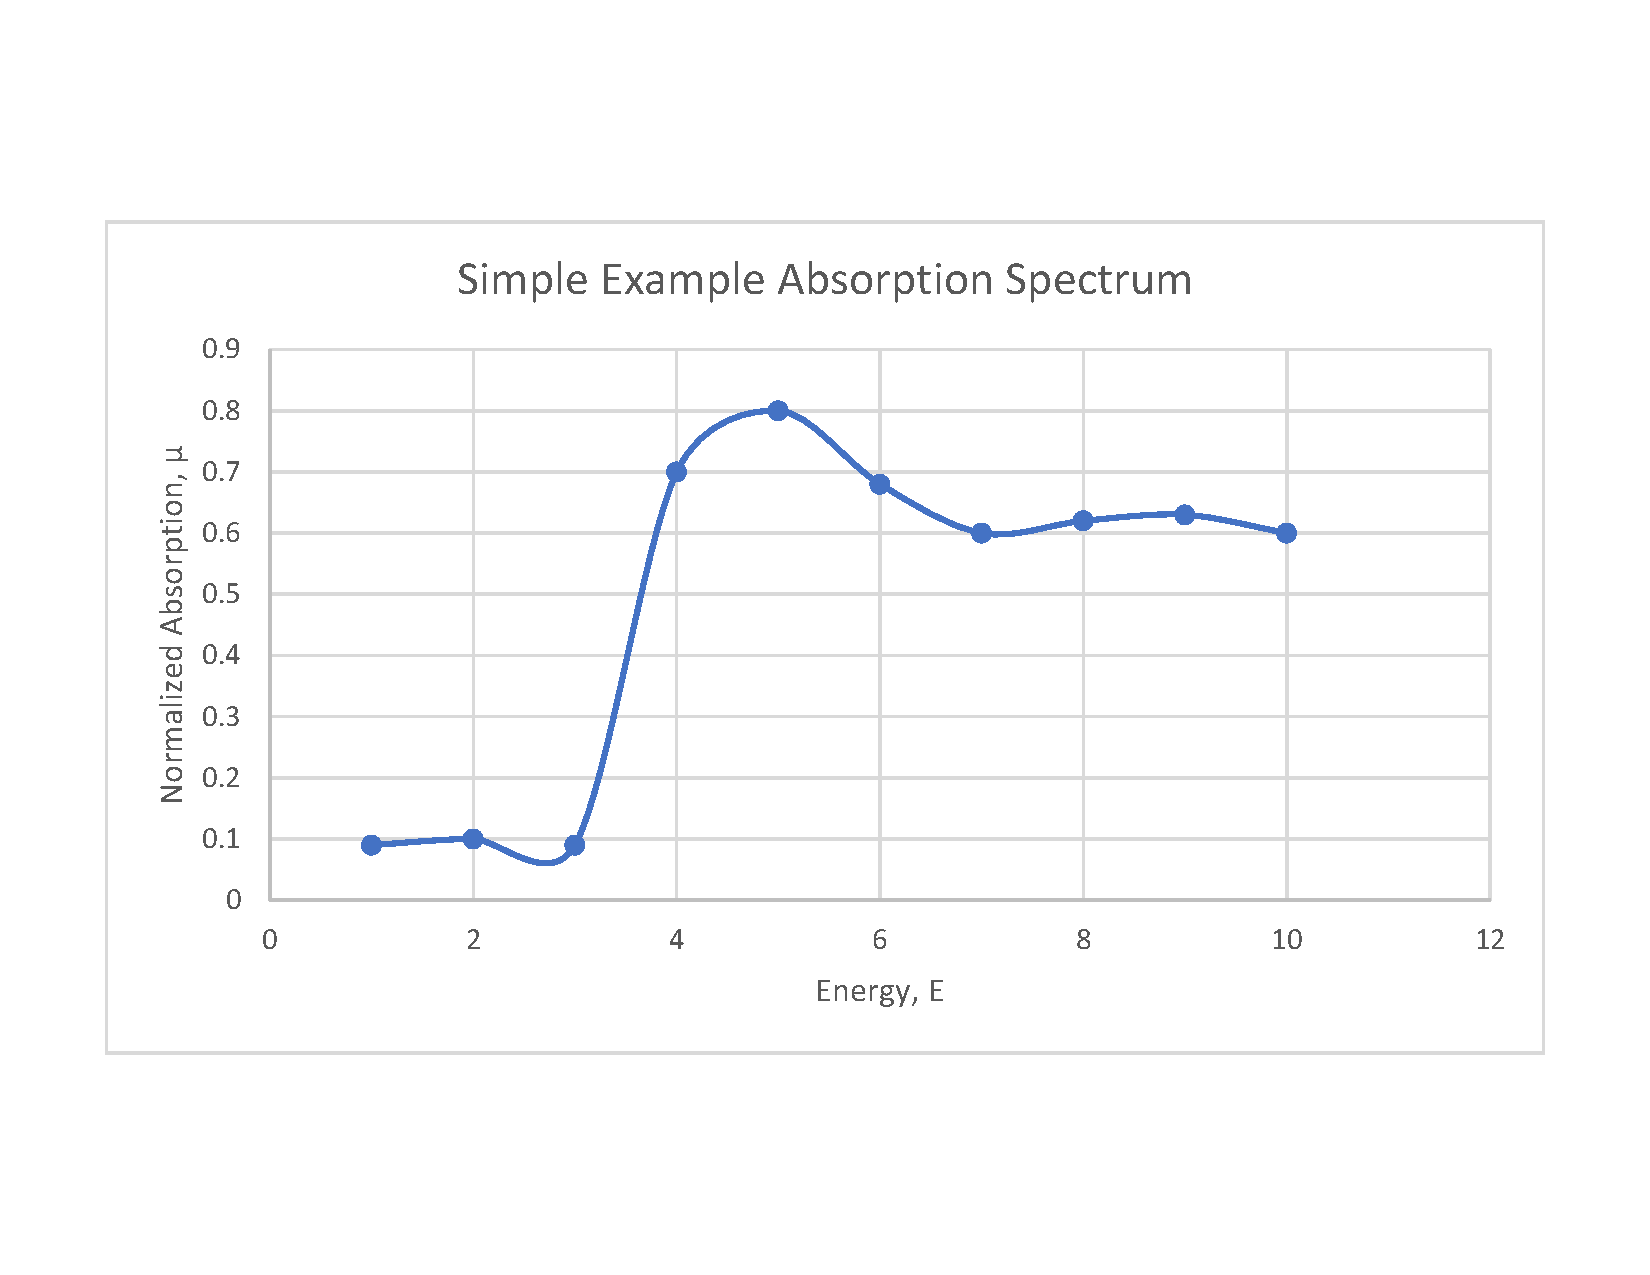
\includegraphics[width=.75\linewidth]{Chapters/Figures/conv-example.pdf}
    \caption[Toy Absorption Spectrum]{A simple abosrption spectrum for demonstration purposes.}
    \label{fig:conv-ex-spectrum}
\end{figure}
 
\noindent Each data point, $ (E, \mu) $ in the spectrum is described as a feature vector, where the feature is the energy value for a given point $ (E, \mu) $. The vector, $ f $,  is depicted below with boxes to represent each element in the vector. Zeros are padded on both sides for reasons that will become clear soon. 

\begin{table}[h!]
    \centering
    \begin{tabular}{c|c|c|c|c|c|c|c|c|c|c|c|c|}
    \cline{2-13}
    \textit{f} = & 0 & .09 & .10 & .09 & .70 & .80 & .68 & .60 & .62 & .63 & .60 & 0 \\ \cline{2-13}
    \end{tabular}
\end{table}

\noindent Additionally, consider the kernel, $ g $  

\begin{table}[h!]
\centering
    \begin{tabular}{lccc}
    \cline{2-4}
    \multicolumn{1}{l|}{\textit{g} =} & \multicolumn{1}{c|}{.1} & \multicolumn{1}{c|}{.1} & \multicolumn{1}{c|}{.1} \\ \cline{2-4}                 
    \end{tabular}
\end{table}

\noindent The convolution works by multiplying each element in the input vector $ f $ by the corresponding element in the kernel $ g $ and summing the results. The kernel then moves to be centered around the next element in $ f $. One way to think about this process is a kernel or filter sliding over an input signal. Applying the kernel $ g $ onto the first index of $ f $ yields: 

\begin{table}[h!]
    \centering
    \begin{tabular}{|c|c|c|c|c|c|c|c|c|c|c|c|}
    \hline
    0  & .09 & .10 & .09 & .70 & \multicolumn{1}{c|}{.80} & \multicolumn{1}{c|}{.68} & \multicolumn{1}{c|}{.60} & .62 & .63 & .60 & 0 \\ \hline
    .1 & .1  & .1  &     &     &                          &                          &                          &     &     &     &   \\ \hline
    \end{tabular}
\end{table}
$$ 
h(1) = (0)(.1) + (.09)(.1) + (.10)(.1) = 0.019
$$

\noindent where $ h(1) $ is 1st index of the resulting vector. For the next point, the kernel shifts to be centered around it. 

\begin{table}[h!]
    \centering
    \begin{tabular}{|c|c|c|c|c|c|c|c|c|c|c|c|}
    \hline
    0 & .09 & .10 & .09 & .70 & \multicolumn{1}{c|}{.80} & \multicolumn{1}{c|}{.68} & \multicolumn{1}{c|}{.60} & .62 & .63 & .60 & 0 \\ \hline
      & .1  & .1  & .1  &     &                          &                          &                          &     &     &     &   \\ \hline
    \end{tabular}
\end{table}

$$ 
h(2) = (.09)(.1) + (.10)(.1) + (.09)(.1) = 0.028
$$

\noindent The final resulting vector is:

\begin{table}[h!]
    \centering
    \begin{tabular}{c|c|c|c|c|c|c|c|c|c|c|}
    \cline{2-11}
    \textit{h} = & .019 & .028 & .089 & .159 & .218 & .208 & .190 & .185 & .185 & .123 \\ \cline{2-11} 
    \end{tabular}
\end{table}

\begin{figure}[h!]
    \label{fig:conv-res-spectrum}
    \centering
    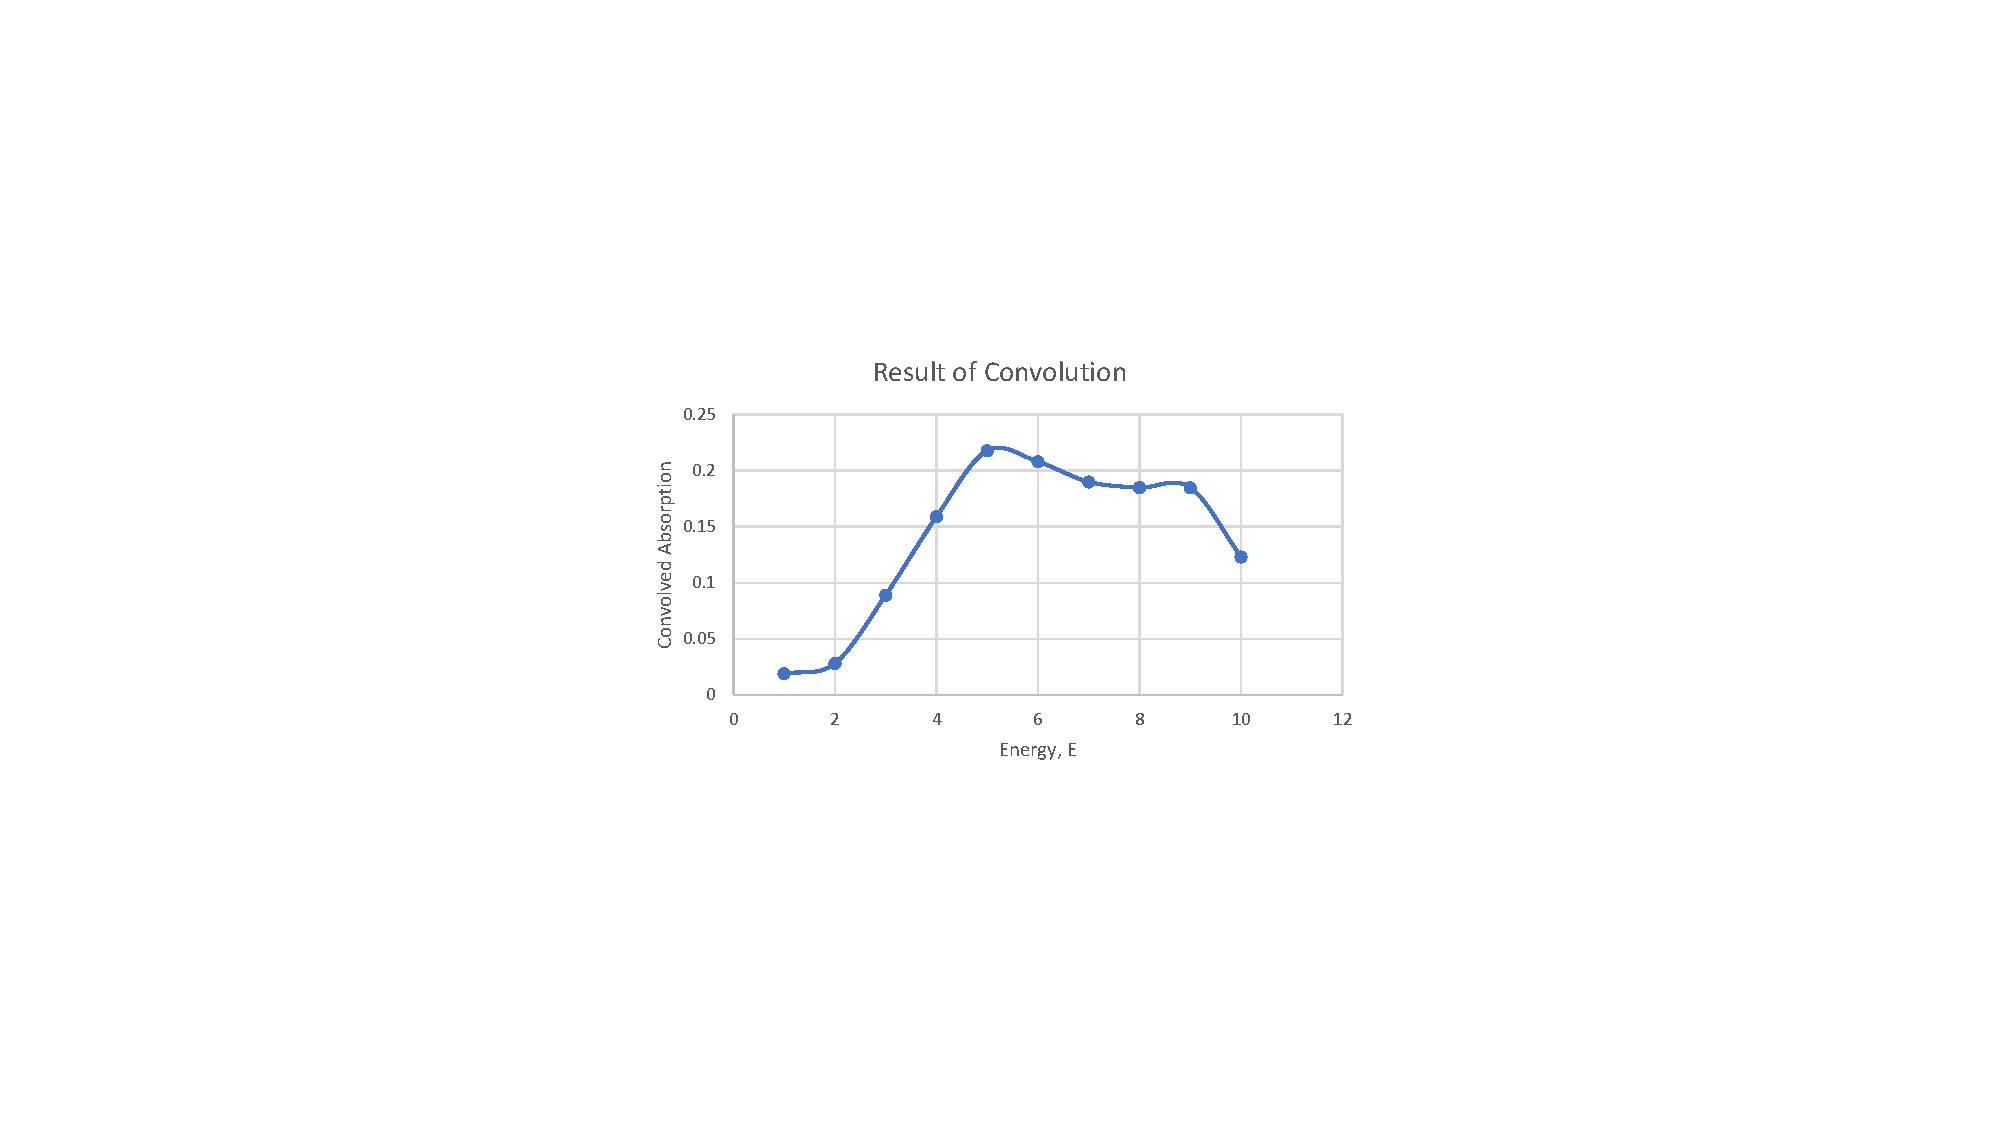
\includegraphics[width=.75\linewidth]{Chapters/Figures/conv-example-res.pdf}
    \caption[1D Convolution Result]{The result of the 1D convolution of kernel $ g = (.1, .1, .1) $  on the spectrum in Figure \ref{fig:conv-ex-spectrum}.}
\end{figure}

The toy example was chosen to demonstrate the basics of a 1D convolution. In this example, the input spectrum was a vector of length ten and the kernel of length three. In the context of applying a 1D convolution to a neural network, the size of the input vector is the cardinality of the hidden layer directly preceding the convolutional layer. Often the hidden layer's output, represented as a vector, is reshaped into an n-dimensional tensor before applying the convolution. To apply a 1D-convolution to a Tensor of rank $ n $, simply apply the convolution to each of the n-vectors separately, ensuring to pad the ends of each vector with zeros. Layers with dimensionality greater than one can be ``un-raveled''. Alternatively, the layers of each dimension can be truncated or ``pooled'' by averaging the layers that are stacked on one another (or taking the max of each layer) until the desired dimensionality is achieved. A common way to achieve this is with a max-pooling layer or an average pooling layer. Max pooling and average pooling layers also have the additional benefit of downsampling the feature space, tending to make the network more robust to slight variations in the position of features in the input image or signal. This is referred to as ``local translation invariance'' \cite{local-translation-invariance}.

Another important possible change in the above example is the stride length. In the above example, we ``slid'' the kernel across the input spectrum one point at a time. This is referred to as a stride size or stride length of one. The stride could be any integer less than the length of the input vector $ f $, though in practice, typically stride lengths tend to be one or close to one. Lastly, in the above example, we only applied one convolutional kernel, or ``filter.'' In practice, many filters are applied sequentially. In the above example, the filter $ g = (.1, .1, .1) $ was simply decided upon \textit{a priori}. In practice, the values for each filter in the convolutional layer are initialized randomly or according to the specified initialization function. The default in Keras is Glorot Uniform. The values of each filter are trainable parameters that evolve to produce the best final prediction given the subsequent layers in the neural network.


\section{How to Train a Neural Network}
Building a successful neural network requires a combination of intuition and procedural know-how. The first key is to start with a simple model, perhaps a single hidden. \textit{If you start with a complex model including data augmentation and regularization, you will never be able to tune the hyperparameters and find a good solution}. A good strategy is to pick a simple architecture and reasonable hyperparameters and train the model on a small subset of training samples, say 1--10 samples. Then, train the model over ten or so epochs and see if the training cost decreases and whether you can overfit it. If you can overfit the small sample size, it means the code is working, and the network architecture makes sense. Now is the time to increase the number of samples in the training data, either to the full train-test split or a subset of if working with ``big data.''\footnote{Big data has become a nebulous term, but a reasonable example is when there is so much data that the dataset cannot be loaded into the computer's memory (RAM) at the same time.} Next, you can run a broad hyperparameter search. Afterward, run maybe 20 epochs and see how the training and validation loss is moving. If they both are going down, the architecture looks good. If not, start over. Ideally, the training and validation loss curves will be decreasing together like in figure \ref{fig:Example-Training-Loss-Curve}. If the model still does not predict well after hyperparameter tuning, the model is underfitting, and a more complex architecture is required (add more layers).

\begin{figure}
    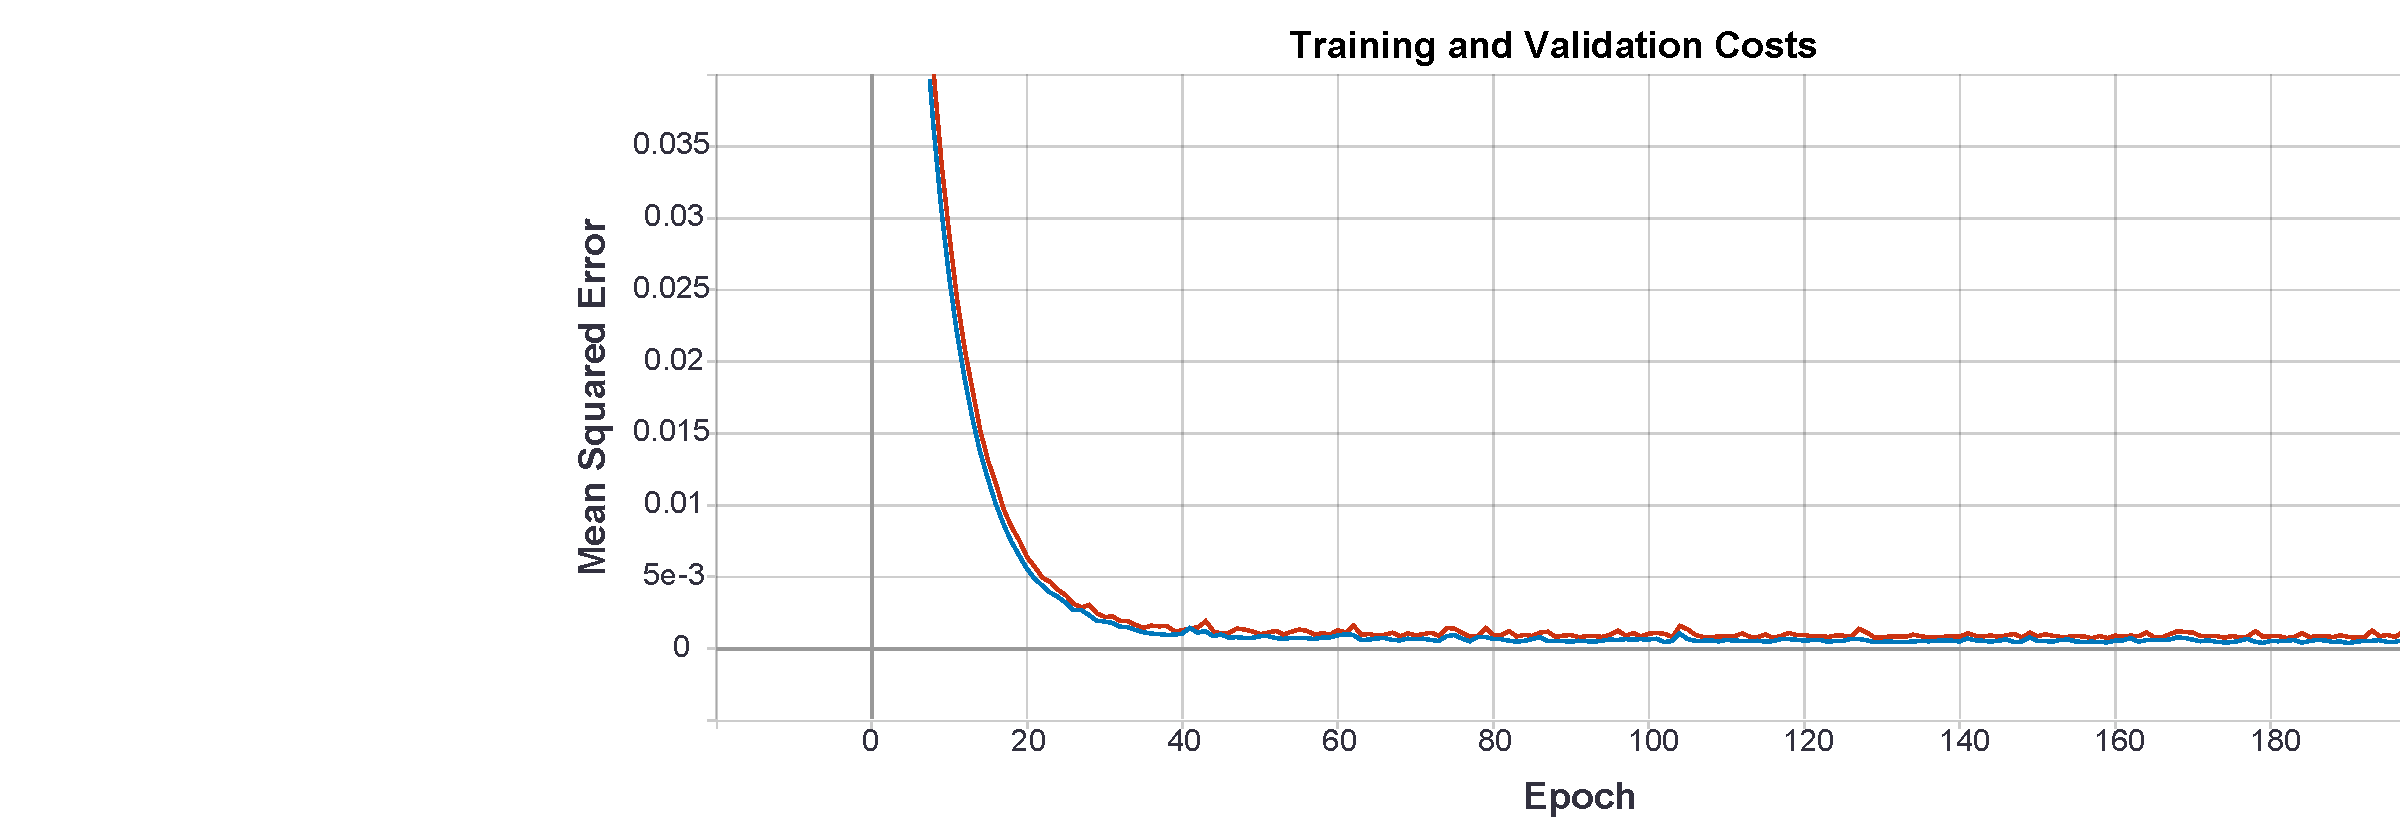
\includegraphics[width=\linewidth]{Chapters/Figures/epoch_loss1.pdf}
    \caption[Example ANN Training Curve]{In this example loss curve, the x-axis is the epoch, and the y-axis is the mean-squared error of the predictions. The red curve is the training data, and the blue curve is the validation set. Notice how both curves decrease together, but the training curve has a smaller error than the validation curve. This is the expected behavior of a model that is not overfitting and training properly.}
    \label{fig:Example-Training-Loss-Curve}
\end{figure}

Ideally, the training and validation loss will decrease together over many epochs. It is likely, however, that after many epochs the training loss will continue to decrease while the validation loss plateaus. This is the point to start introducing regularization such as dropout layers as well and considering data augmentation. These techniques will allow the model to continue decreasing the validation loss and prevent overfitting. The main goal of training is to minimize the validation loss. The placement of dropout layers and the type of data augmentation are subject to trial and error. Generally, it is best to include dropout layers after a ReLU activation and before an affine layer. There has been some research suggesting the inclusion of low-probability dropout layers after convolutional layers tends to improve model performance \cite{conv-dropout-layers} \cite{conv-dropout-layers2}, but these rules do not work for every network, and it is still worth trying many options while training.



% \section{Autoencoders if they become useful}
% Talk about how autoencoders work. Give a nice broad explanation and really go into the math. Include some nice diagrams

% Here's \cite{ng2011sparse} a good source to read and model off of. Here \cite{Bhowick2019} is another paper that might be interesting to read. It's about getting noise-free data from the original data using an autoencoder. Neat idea, and could actually be very relevant because they're using geophysical data.



